%TEX
% Sun Nov 07 12:04:37 EST 2021
% ++++++++++++++++++++++++++++++++++++++++++++++++++
% North American GeoGebra Journal LaTeX template file.  
%            :  Template Control File  
%            :  
%            :  LaTeX environment. Read the README.md file
%            :  Note configs.tex file for packages.  
%            :  MIT License.
%            :
%            : Quinlan, J. 
% ++++++++++++++++++++++++++++++++++++++++++++++++++
% FOR ASSISTANCE TRY: 
%           : http://en.wikibooks.org/wiki/LaTeX/
%           : https://www.ctan.org/
%              

\def\pagenum{1}
\def\vol{1}
\def\issue{1}

% ----------------------------- %
%  \listfiles
% \documentclass[fleqn,12pt]{article}
\documentclass[12pt]{article}

%\usepackage{authblk}
%\setlength{\affilsep}{0em}
\usepackage{times}                                     
\usepackage{amsfonts,amsmath,amssymb} 

% \setlength{\mathindent}{0pt}
\usepackage{amsthm}
\usepackage{latexsym}
\usepackage[a4paper]{geometry}    



\usepackage{fancyhdr}
\usepackage{placeins}                           
\usepackage{xcolor}
\usepackage[utf8]{inputenc} % Character encoding
\usepackage{graphicx}%
\usepackage{tabularx}
\usepackage{array}
\newcolumntype{x}[1]{%
>{\raggedleft\hspace{0pt}}p{#1}}%

%\usepackage{hyperref}
%\usepackage[hidelinks]{hyperref}
%\usepackage[hyphens]{url}

%\usepackage{etoolbox}
%\usepackage[shortlabels]{enumitem}
%\usepackage[normalem]{ulem}  % strike through text

% Book Tables
\usepackage{booktabs}

\usepackage{comment}
% \input{macros}
% USE THIS TO CHANGE THE SPACING BETWEEN TABLES AND CAPTIONS!!!
\usepackage[labelfont=bf,labelsep=period, skip=5pt]{caption}
 
% TiKz
\usepackage{pgf,tikz}
\usepackage{mathrsfs}
\usetikzlibrary{arrows}

% PDF Plots
\usepackage{pgfplots}
\pgfplotsset{width=7cm,compat=1.10}

% For side-by-side figures
\usepackage{caption}
\usepackage{subcaption}
\usepackage{float}

% Editing: highlight and strikethru
\usepackage{soul}
% \usepackage{todonotes}  % editing (make comments \todo{X}
%\usepackage{lipsum}

% OUTLINES
\usepackage{outlines}
\usepackage{enumitem}
\setenumerate[1]{label=\arabic*.}
\setenumerate[2]{label=(\alph*).}
\setenumerate[3]{label=\roman*.}
\setenumerate[4]{label=\alph*.}

% Citations and References
% https://merkel.texture.rocks/Latex/natbib.php
\usepackage[authoryear, round]{natbib}


\makeatletter
\renewcommand\@biblabel[1]{}
\renewenvironment{thebibliography}[1]
     {\section*{\refname}%
      \@mkboth{\MakeUppercase\refname}{\MakeUppercase\refname}%
      \list{}%
           {\leftmargin0pt
            \@openbib@code
            \usecounter{enumiv}}%
      \sloppy
      \clubpenalty4000
      \@clubpenalty \clubpenalty
      \widowpenalty4000%
      \sfcode`\.\@m}
     {\def\@noitemerr
       {\@latex@warning{Empty `thebibliography' environment}}%
      \endlist}
\makeatother




\RequirePackage{color}
\definecolor{cej@color}{rgb}{0.5,0.37109375,0.59765625}
\definecolor{abs}{rgb}{0.251,0.541,0.72.9}
\definecolor{ffqqqq}{rgb}{1,0,0}
\definecolor{qqqqff}{rgb}{0,0,1}
\definecolor{cqcqcq}{rgb}{0.75,0.75,0.75}
\definecolor{ttqqqq}{rgb}{0.2,0,0}
\definecolor{ffxfqq}{rgb}{1,0.5,0}
\definecolor{uuuuuu}{rgb}{0.27,0.27,0.27}
\definecolor{ffqqff}{rgb}{1,0,1}
\definecolor{xfqqff}{rgb}{0.5,0,1}
\definecolor{xdxdff}{rgb}{0.49,0.49,1}
\definecolor{red}{rgb}{1,0,0}
\definecolor{blue}{rgb}{0,0,1}
\definecolor{ccqqqq}{rgb}{0.8,0,0}
\definecolor{fftttt}{rgb}{1,0.2,0.2}
\definecolor{qqwuqq}{rgb}{0,0.39,0}
\definecolor{qqqqff}{rgb}{0,0,1}
\definecolor{wrwrwr}{rgb}{0.3803921568627451,0.3803921568627451,0.3803921568627451}
\definecolor{sexdts}{rgb}{0.1803921568627451,0.49019607843137253,0.19607843137254902}
\definecolor{rvwvcq}{rgb}{0.08235294117647059,0.396078431372549,0.7529411764705882}
\definecolor{ccqqqq}{rgb}{0.8,0,0}
\definecolor{qqqqff}{rgb}{0,0,1}
\definecolor{wwwwww}{rgb}{0.4,0.4,0.4}
\definecolor{qqwuqq}{rgb}{0,0.39215686274509803,0}
\definecolor{uuuuuu}{rgb}{0.266,0.266,0.266}

% Allows customization of titles
\usepackage{titlesec}
\titleformat{\section}[block]{\normalsize\scshape\bfseries{\arabic{section}.}}{}{1em}{}
\titleformat{\section}[block]{\normalsize\scshape\bfseries}{\thesection}{1em}{}
\titleformat*{\subsection}{\normalsize\scshape\itshape\bfseries}
\titleformat*{\subsubsection}{\smallsize\scshape\itshape}
\usepackage{framed}
% \usepackage[hyphens]{url}
%\usepackage[hyphens,spaces,obeyspaces]{url}
% \usepackage[colorlinks,allcolors=blue]{hyperref}
\usepackage[colorlinks,allcolors=black]{hyperref}
\newtheorem{theorem}{Theorem}%[section]      
\newtheorem{acknowledgement}[theorem]{Acknowledgement}
\newtheorem{algorithm}[theorem]{Algorithm}  
\newtheorem{axiom}[theorem]{Axiom} 
\newtheorem{case}[theorem]{Case}
\newtheorem{claim}[theorem]{Claim}     %
\newtheorem{conclusion}[theorem]{Conclusion}
\newtheorem{condition}[theorem]{Condition}
\newtheorem{conjecture}[theorem]{Conjecture}
\newtheorem{corollary}[theorem]{Corollary} 
\newtheorem{criterion}[theorem]{Criterion} 
\newtheorem{definition}[theorem]{Definition}
\newtheorem{example}{Example}
\newtheorem{exercise}[theorem]{Exercise}
\newtheorem{lemma}[theorem]{Lemma}
\newtheorem{notation}[theorem]{Notation}
\newtheorem{problem}[theorem]{Problem}
\newtheorem{question}[theorem]{Question}
\newtheorem{questions}{Question}
\newtheorem{questionsa}{Question}
\newtheorem{questionsb}{Question}                   %
\newtheorem{proposition}[theorem]{Proposition}
\newtheorem{remark}[theorem]{Remark}
\newtheorem{solution}[theorem]{Solution}
\newtheorem{summary}[theorem]{Summary}



\setcounter{page}{\pagenum}
\newcounter{ggbFirstpage}
\setcounter{ggbFirstpage}{\pagenum}
\pagestyle{empty}
\setlength{\headheight}{14pt}
\geometry{left=2cm,right=2cm,top=3cm,bottom=3cm}
\pagestyle{fancyplain}                              

\fancyhf{}
\fancyhead[c]{\small \emph{North American GeoGebra Journal}%
\, Volume \vol, Number \issue, ISSN 2162-3856}     %
\cfoot{%                                            
  \ifnum\value{ggbFirstpage}=\pagenum%              
    {\vtop to\hsize{\hrule\vskip .2cm {\thepage}}}%   = the starting page number         %
  \else\setcounter{ggbFirstpage}{\pagenum}\fi%      
}                                                   

\newcommand*{\TitleFont}{%
      \usefont{\encodingdefault}{\rmdefault}{}{n}%
      \fontsize{16}{18}%
      \selectfont}

\def\authorfont{\normalfont\fontsize{12}{14}\selectfont\centering}
\def\subauthorfont{\normalfont\fontsize{10}{12}\selectfont\centering}
\definecolor{wrwrwr}{rgb}{0.3803921568627451,0.3803921568627451,0.3803921568627451}
\definecolor{sexdts}{rgb}{0.1803921568627451,0.49019607843137253,0.19607843137254902}
\definecolor{rvwvcq}{rgb}{0.08235294117647059,0.396078431372549,0.7529411764705882}
\bibpunct[, ]{(}{)}{;}{a}{,}{,}


%\usepackage{mfirstuc}
% https://www.titlecase.com



 

%Display code in article
\usepackage{listings}
\usepackage{textcomp}
\usepackage{xcolor}
 \lstset{ 
  backgroundcolor=\color{white},  % background color; e.g., nearwhite you must add \usepackage{color} or \usepackage{xcolor}; should come as last argument
  basicstyle=\footnotesize\ttfamily,% the size of the fonts that are used for the code
  breakatwhitespace=false,% sets if automatic breaks should only happen at whitespace
  breaklines=true, % sets automatic line breaking
  framextopmargin=5pt,
  framexleftmargin=5pt, 
  framexbottommargin=5pt,
  framexrightmargin=0pt,
  framesep=0pt,
  captionpos=b,% sets the caption-position to bottom
  commentstyle=\color{mygreen}, % comment style
  morecomment=[s]{/*}{*/},
  deletekeywords={...}, % if want to delete keywords from the given language
  escapeinside={\%*}{*)},% if you want to add LaTeX within your code
  extendedchars=true,% lets you use non-ASCII characters; for 8-bits encodings only, does not work with UTF-8
  frame=single,	% adds a frame around the code
  keepspaces=false, % keeps spaces in text, useful for keeping indentation of code (possibly needs columns=flexible)
  keywordstyle=\color{blue},% keyword style blue
  language=java, % the language of the code
  morekeywords={},% if you want to add more keywords to the set
  numbers=none, % where line-numbers put; possible values are (none, left, right)
  numbersep=0pt,% how far the line-numbers are from the code
  numberstyle=\tiny\color{mygray}, % the style that is used for the line-numbers
  rulecolor=\color{gray},  % appleGray     % if not set, the frame-color may be changed on line-breaks within not-black text (e.g. comments (green here))
  sensitive=true,
  showspaces=false, % show spaces everywhere adding particular underscores; it overrides 'showstringspaces'
  showstringspaces=false,% underline spaces within strings only
  showtabs=false, % show tabs within strings adding particular underscores
  stepnumber=2,	% the step between two line-numbers. If it's 1, each line will be numbered
  stringstyle=\color{purple}, % string literal style
  tabsize=4,% sets default tabsize to 2 spaces
  title=\lstname, % show the filename of files included with \lstinputlisting; also try caption instead of title
  upquote=true,      % Straight quotes
  belowcaptionskip=0em,
  belowskip=0em
}

% ----------------------------- &


\usepackage{authblk}
\renewcommand\Authands{ and }


% Edit 33 - 37
\def\thetitle{\uppercase{Title of the work}} 
\def\authorOne{\authorfont{John Jones}}
\def\authorTwo{\authorfont{Steve Smith}}
\def\institutionOne{\subauthorfont{Department of Mathematics, Great State University}}
\def\institutionTwo{\subauthorfont{School of Typesetting and Print, \LaTeX\ University}}

% ----------------------------- %
\begin{document}
% ----------------------------- %
\interfootnotelinepenalty=100000


% ----------------------------- %
%  Header: Title, author
% ----------------------------- %
\title{\TitleFont{\thetitle}}
\author[1]{\authorOne}
\author[2]{\authorTwo}
%\author[1]{Author C}
%\author[2]{Author D}
%\author[2]{Author E}
\affil[1]{\institutionOne}
\affil[2]{\institutionTwo}

% Title Placment
\vspace{-1mm}
\date{}                                                 
\maketitle                                              


% ----------------------------- %
% Abstract
% ----------------------------- %
% Abstract and Keywords
%
\bgroup
\color{abs}
\hrule
\egroup
%
%%  DO NOT EDIT LINES ABOVE              

\begin{abstract}
\noindent \textit{The abstract is a single-paragraph summary of approximately 150 to
250 words.  Include a sentence about the focus of the paper and the results, if applicable.  Follow the abstract by three to five keywords (see below).
}\\

\noindent\textbf{Keywords}: Keyword1, Keyword2, Keyword3

\end{abstract}%

\bgroup
\color{abs}
\hrule
\egroup



\thispagestyle{fancy}


% ----------------------------- %
% Sections
% ----------------------------- %
% ----------------------------- %
% Author Guidelines
% ----------------------------- %
\section{General Guidelines}

\noindent Please read these instructions carefully.   The objective of this template is to enable you in an easy way to style your article attractively in a style similar to that of the typeset journal. It should be emphasized, however, that the final appearance of your paper in print and in electronic media may likely vary to some extent from the presentation achieved in this template.


% ----------------------------- %
% Heading Levels
% ----------------------------- %
\subsection{Level Headings: Subsections}
\noindent You will usually want to divide your article into (numbered) sections and subsections (perhaps even subsubsections).  Use to help organize your document as appropriate.


% ----------------------------- %
% Paragraphs
% ----------------------------- %
\subsection{Paragraphs}
\noindent Paragraphs are \textbf{not} indented and a line break is included between paragraphs.  The first paragraph in a section or subsection will automatically  not  have an indentation.  Use \verb!\noindent! as needed.  


% ----------------------------- %
% Hyperlinks
% ----------------------------- %
\subsection{Hyperlinks / URLs} 
Include hyperlinks using  URL \url{http://www.google.com}.  


% ----------------------------- %
% Mathematics
% ----------------------------- %
\section{Mathematics}\label{sec:lu}
Here is some mathematics.  For $A \in M_n$, the factorization $A = LU$, where $L$ is unit lower triangular and $U$ is upper triangular,  is called the \textit{LU decomposition}, or \textit{LU factorization}.  We can use such a factorization, when it exists, to solve the system $A {\bf x} = {\bf b}$ by first solving for the vector $\bf{y}$ in $L {\bf y} = {\bf b}$ 
and then solving 
$
U {\bf x} = {\bf y}
$. 
However, not every $n \times n$ matrix $A$ has an LU decomposition.  The following theorem provides conditions for the existence and uniqueness of an LU decomposition of a $n \times n$ matrix.  A proof can be found in \citet[p. 160]{johnson1985matrix}.  An equation is given by \cite{strang1993introduction}, 

\begin{equation}\label{eqn:quad}
x = \frac{-b \pm \sqrt{b^2 - 4ac}}{2a}
\end{equation}
  
%: EXAMPLE 1
\begin{example}\normalfont
The $3 \times 3$ matrix  
$A =  \begin{bmatrix}
1 & 5 & 1\\
1 & 4 & 2\\
4 & 10 & 2\\
\end{bmatrix}
$
has all non-zero principle minors, $A_1, A_2$ and $A_3$.  Therefore,  there is a unique LU factorization with both $L$ and $U$ nonsingular given by 
\end{example}
\[
\begin{bmatrix}
1 & 5 & 1\\
1 & 4 & 2\\
4 & 10 & 2\\
\end{bmatrix}
=
\begin{bmatrix}
1 & 0 & 0\\
1 & 1 & 0\\
4 & 10 & 1\\
\end{bmatrix}
\begin{bmatrix}
1 & 5 & 1\\
0 & -1 & 1\\
0 & 0 & 12\\
\end{bmatrix}.
\]



% ----------------------------- %
% Math: Theorems/Defs
% ----------------------------- %
\section{Definition, Theorem, Corollary}


\begin{definition}
Definitions are if and only if statements.  
\end{definition}

\begin{verbatim}
\begin{definition}
Definitions are if and only if statements.  
\end{definition}
\end{verbatim}

%: THEOREM: Infinite LU Factorizations
\begin{theorem}[Matrices with Infinitely Many LU Factorizations]
{For $A \in M_n$, if two or more of any first $(n-1)$ columns are linearly dependent or any of the first $(n-1)$ columns are 0, then $A$ has infinitely many LU factorizations.}
\end{theorem}

%: proof
\begin{proof} We will prove only for the the case when $A \in M_3$. \\
 \begin{align} 
&dm + r = e  \Rightarrow r = e-dm \label{eqn:1}\\
&dn + rp = f \Rightarrow p=\frac{f-dn}{r} \label{eqn:2}\\
&gm + s = h \Rightarrow s = h - gm \label{eqn:3}\\
&gn + sp + t = i \Rightarrow t  = i-sp-gn \label{eqn:4}
\end{align}
 
\end{proof} % end proof
 

% Corollary
\begin{corollary}
If $x$, then $y$.
\end{corollary}



% ----------------------------- %
% Examples
% ----------------------------- %
\section{Examples}\label{ex:x1}
Here is an example of an example.


\begin{example}
Let  $\{1,2,3\}$ and $\{2,1,3\}$ be two lists of integers.  Then, to check if the two lists are equal we would have,   
	\begin{center}
		\texttt{ \{1,2,3\} == \{2,1,3\} }.
	\end{center}\label{ex:equallists}
\end{example}


\begin{verbatim}
\begin{example}
Let  $\{1,2,3\}$ and $\{2,1,3\}$ be two lists of integers.  Then, to check if the two lists are equal we would have,   
	\begin{center}
		\texttt{ \{1,2,3\} == \{2,1,3\} }.
	\end{center}\label{ex:equallists}
\end{example}
\end{verbatim}



% ----------------------------- %
% Lists
% ----------------------------- %
 \section{Lists}
 NAGJ uses the \verb|outline| package.   
  
 % Enumeration
 \subsection{Enumerated List}
 The following code produces an enumerated list.  The enumerated list numbers each list item with Arabic numerals.
 
% Outline
\begin{verbatim}
\begin{outline}[enumerate]
     \1 First Level
          \2 Second level
               \3 Third level
\end{outline}
 \end{verbatim}
 
 % Outline
 \begin{outline}[enumerate]
 	\1 First Level
		\2 Second level
			\3 Third level
\end{outline}
 

 % Itemize
 \subsection{Itemized List}
 The following code produces an itemized list.
 
% Verbatim Outline
\begin{verbatim}
\begin{outline}
     \1 First item
          \2 Second level item
               \3 Third level sub-item
\end{outline}
 \end{verbatim}
 
 % Outline
 \begin{outline}
 	\1 First Level
		\2 Second level
			\3 Third level
\end{outline}



% ----------------------------- %
% Tables and Figures
% ----------------------------- %
\section{Tables and Figures}

A \textbf{caption} that briefly describes the material is required for figures and tables.  Any required information, such as photo credits or data source, may be included in captions. Furthermore, as part of the authorization to use that content, providers of this material may need a specific credit line, which might be placed in the caption (or wherever the provider has requested).  


% ----------------------------- %
% Figures
% ----------------------------- %
 \subsection{Figures}
Figures should be high quality (1200 dpi for line art, 600 dpi for grayscale and 300 dpi for color, at the correct size). The preferred method of including graphics in the \textit{North American GeoGebra Journal} is to export to TiKz.  For exposition on TiKz, see \citep{quinlan2013geogebra}.   
Other acceptable file formats include: EPS, PS, PNG, JPEG, or TIFF.  
  
 \begin{figure}[h!] %  figure placement
    \centering
    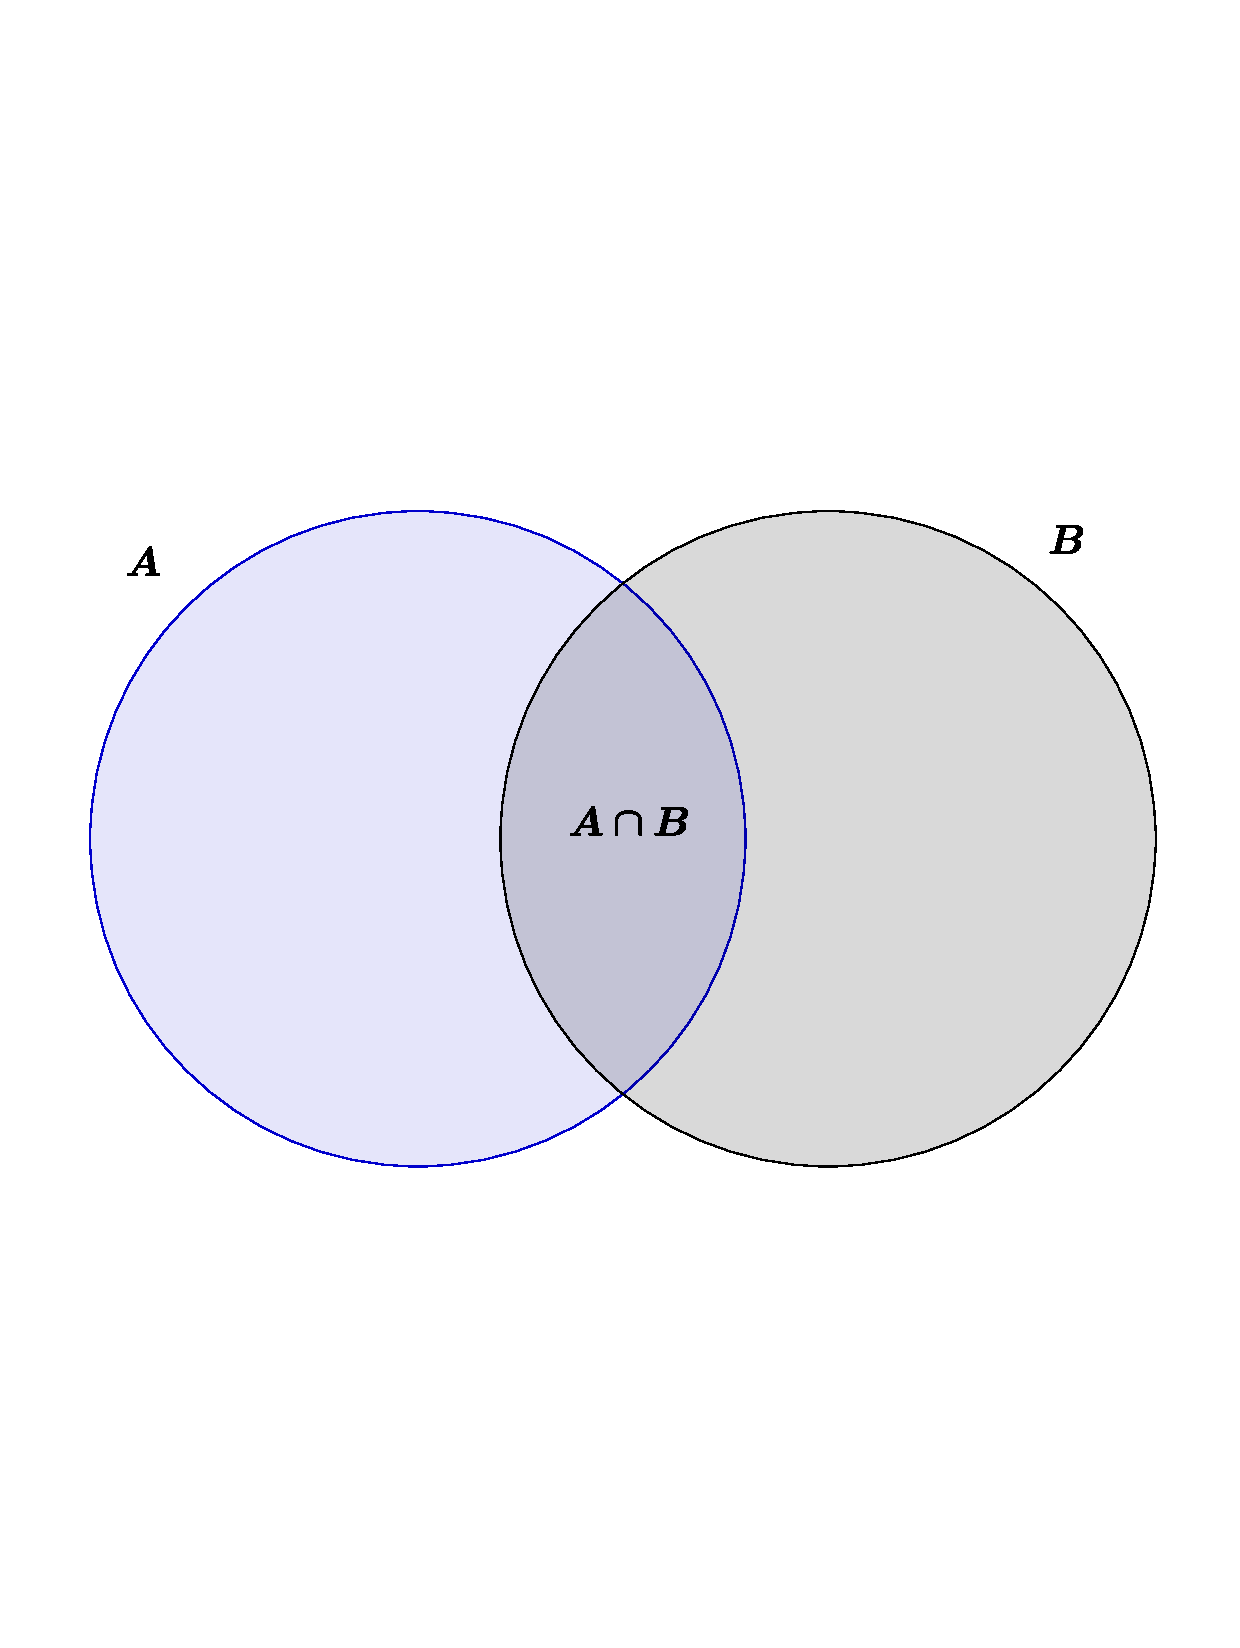
\includegraphics[scale=0.5]{figs/venn.pdf} 
    \caption{Provide a short caption description.}
    \label{fig:number}
 \end{figure}
 
 
% ----------------------------- %
% Tables
% ----------------------------- %
\subsection{Tables}
We use the \texttt{booktabs} package.  Tables should present new information rather than duplicating what is in the text. Readers should be able to interpret the table without reference to the text. Please supply editable files.


\begin{table}[ht!]
\begin{center}
\begin{tabular}{lccc} 
	\toprule
	Date & Time  &  Average   & Standard Deviation \\ 
	\midrule
	Jan 1  & 1100	& 4.7		& 0.6		\\
	Jan 2  & 2300	& 16.7	& 2.9		\\
	Jan 3  & 1400	& 11.4	& 3.5		\\
	Jan 4  & 1130	& 8.4		& 2.1		\\
	Jan 5  & 500	& 5.2		& 1.9		\\
	Jan 6  & 1700	& 7.9		& 2.2		\\
	\bottomrule 
\end{tabular} 
\caption{This is a caption to the table}
\label{tab:1} 
\end{center}
\end{table} % end the table



% ----------------------------- %
% Cross Referencing
% ----------------------------- %
\section{Cross Reference}
Figures, tables, and equations should be labeled (\texttt{label}) then referenced using the \texttt{ref}. 


% ----------------------------- %
% Citations
% ----------------------------- %
\section{Citations}
Citations follow APA format.  \citet{johnson1985matrix} shows an example using \verb!\citet{key}!, whereas to include citations parenthetically as in, \citep{johnson1985matrix}, use \verb!\citep{key}!.  You can also include page number of reference such as, \citep[p. 17]{johnson1985matrix}, by using options in the cite command, i.e.,  \verb!\citep[p. 17]{key}!.  Multiple researchers \citep{johnson1985matrix,strang1993introduction} can be cited using one cite command; in particular, with keys separated by commas  \verb!\citep{johnson1985matrix,strang1993introduction}!.



% ----------------------------- %
% GeoGebra Commands
% ----------------------------- %
\section{GeoGebra Command Line}
Commands that could be entered at the GeoGebra command prompt should use the \verb!verbatim! environment and can be centered.
\begin{center}
\verb! J=(6-(16/3-distance(D,K)),y(C)).!
\end{center}
For inline commands such as \texttt{distance(A,B)}, use \verb!\texttt! or \verb!\verb!.   


% ----------------------------- %
% Appendix
% ----------------------------- %
\section*{Appendix}
Appendixes, if needed, appear before the acknowledgment.



% ----------------------------- %
% Acknowledgment
% ----------------------------- %
\section*{Acknowledgment}
The preferred spelling of the word ``acknowledgment" in American English is without an ``e" after the ``g." Use the singular heading even if you have many acknowledgments. Avoid expressions such as ``One of us (S.B.A.) would like to thank ... ." Instead, write ``F. A. Author thanks ... ." In most cases, sponsor and financial support acknowledgments are placed in the unnumbered footnote on the first page, not here.





% ----------------------------- %
% References:  BibTeX
% ----------------------------- %
\bibliography{refs.bib}
\bibliographystyle{apalike}


% ----------------------------- %
% Biography
% ----------------------------- %
\noindent
\fbox{
\begin{tabular}{m{0.15\textwidth} m{0.78\textwidth} }
\vspace{0.2cm}
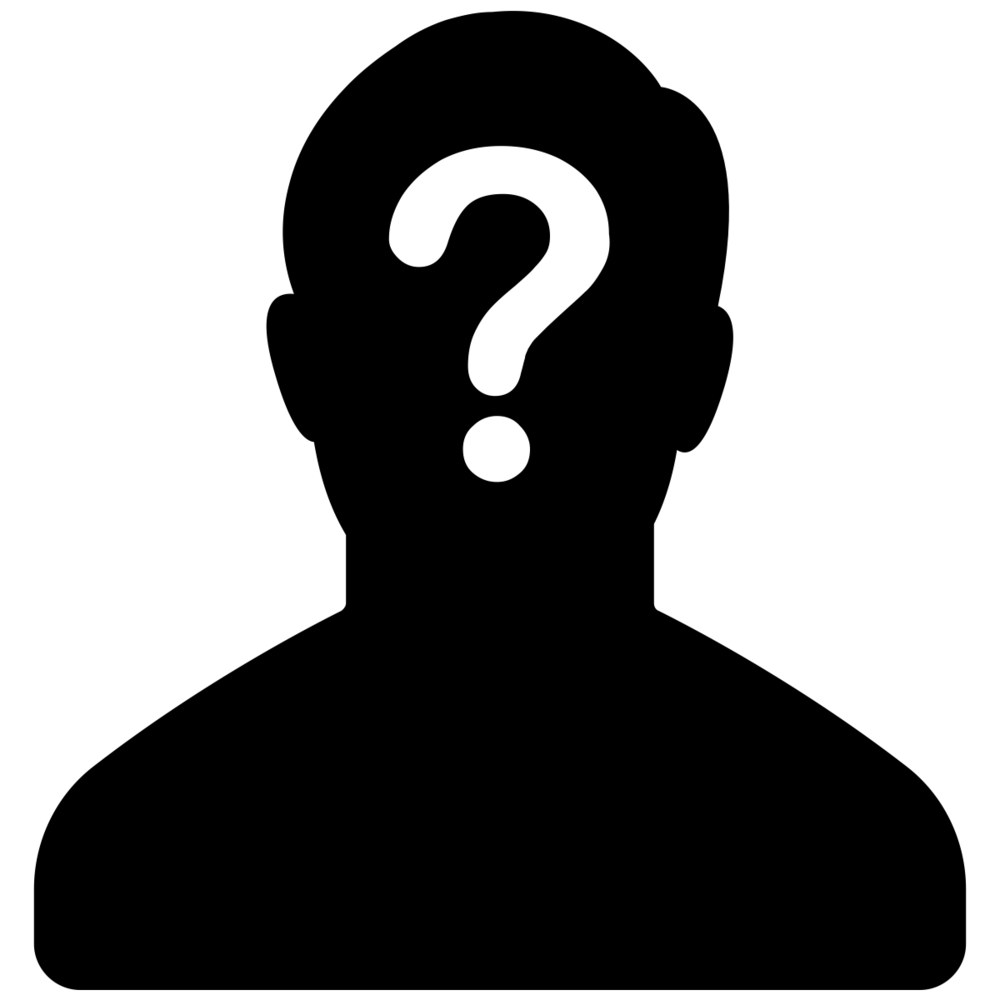
\includegraphics[width=.15\textwidth]{figs/author1.png}
&
\textbf{Author} is an Associate Professor at all the best universities.  
\end{tabular}
}
\newline
\\\\
\noindent
\fbox{
\begin{tabular}{m{0.15\textwidth} m{0.78\textwidth} }
\vspace{0.2cm}
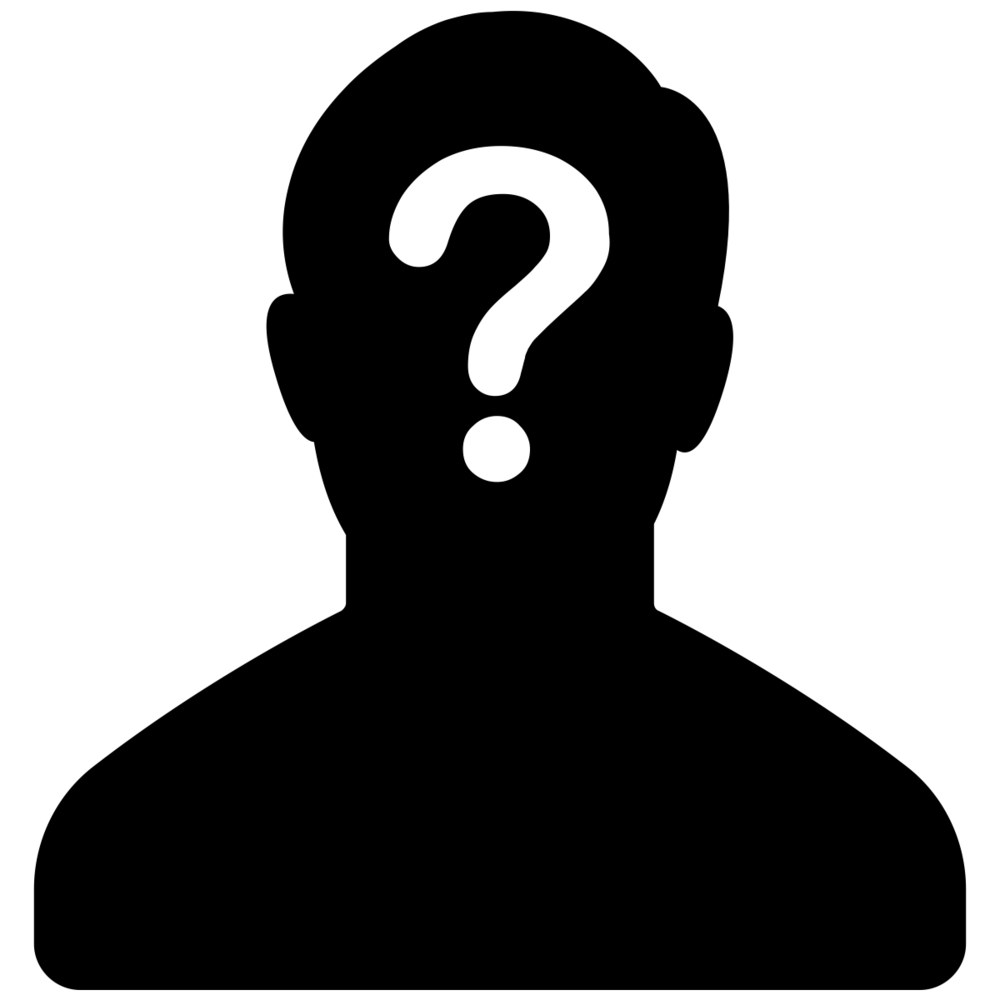
\includegraphics[width=.15\textwidth]{figs/author2.png}
&
\textbf{Author},  is a professor and has taught you everything you know.  
\end{tabular}
}



% ----------------------------- %
% Appendix: If needed
% ----------------------------- %
\newpage

%: SECTION - LU Decomposition CODE

\section*{Appendix - Code}

\begin{lstlisting}
for(int i = 0; i < dim - 1; i++){
	for(int k = i+1; k  < dim; k++ ){
		for(int m =  i+1; m < dim; m++){
			if(upper[i][i] == 0 && upper[m][i] != 0 ){
				'THERE IS NO LU FACTORIZATION'
            }
        }
		if(upper[i][i] != 0 && upper[k][i] != 0){
	        multiplier =upper[i][i]/upper[k][i];
	        lower[k][i] = multiplier;
        }else{
	        if(upper[i][i] == 0 && upper[k][i] == 0){
		        INFINITELY MANY LU FACTORIZATIONS 
		        multiplier = INPUT FROM USER;
		        lower[k][i] = multiplier;
            }
        }
    for(int j = 0; j < dim; j++){
        row[j] = upper[i][j]*multiplier;
    }
    for(int r = 0; r < dim; r++){
        upper[k][r] = upper[k][r] - row[r];
    }
}
Display Lower And Upper
(Perform Matrix Multiplication on L and U)
Display L and U
}
\end{lstlisting}



\end{document} 
